%%%%%%%%%%%%%%%%%%%%%%%%%%%%%%%%%%%%%%%%%%%%%%%%%%%%%%%%%%%%%%%%%%%%%%%%%%%%%%%%
%2345678901234567890123456789012345678901234567890123456789012345678901234567890
%        1         2         3         4         5         6         7         8

\documentclass[letterpaper, 10 pt, conference]{ieeeconf}  % Comment this line out if you need a4paper
\usepackage[utf8]{inputenc}
\usepackage{graphicx}
\usepackage{amsmath}
\usepackage{hyperref}
\usepackage{cleveref}
\usepackage{amssymb}
\usepackage[table]{xcolor}% http://ctan.org/pkg/xcolor
\usepackage{xcolor}
\usepackage{epsfig}
\let\labelindent\relax
\usepackage{enumitem}
\usepackage{pgf,tikz}
\usetikzlibrary{decorations.pathreplacing,calligraphy}
\usepackage{makecell}
\usepackage{mdframed}% http://ctan.org/pkg/mdframed
%\usepackage{geometry}

%\documentclass[a4paper, 10pt, conference]{ieeeconf}      % Use this line for a4 paper

\IEEEoverridecommandlockouts                              % This command is only needed if 
% you want to use the \thanks command

\overrideIEEEmargins                                      % Needed to meet printer requirements.

%In case you encounter the following error:
%Error 1010 The PDF file may be corrupt (unable to open PDF file) OR
%Error 1000 An error occurred while parsing a contents stream. Unable to analyze the PDF file.
%This is a known problem with pdfLaTeX conversion filter. The file cannot be opened with acrobat reader
%Please use one of the alternatives below to circumvent this error by uncommenting one or the other
%\pdfobjcompresslevel=0
%\pdfminorversion=4

% See the \addtolength command later in the file to balance the column lengths
% on the last page of the document

% The following packages can be found on http:\\www.ctan.org
%\usepackage{graphics} % for pdf, bitmapped graphics files
%\usepackage{epsfig} % for postscript graphics files
%\usepackage{mathptmx} % assumes new font selection scheme installed
%\usepackage{times} % assumes new font selection scheme installed
%\usepackage{amsmath} % assumes amsmath package installed
%\usepackage{amssymb}  % assumes amsmath package installed

%\title{\LARGE \bf
%	JAEGO : Attention Sharing in Sensory Egocentric Spheres
%}
%\title{\LARGE \bf
%	From Egocentric Sensory Sphere to Joint Attention and Back 
%}
\title{\LARGE \bf
	%JA-EGO: The Egocentric Dimension of Joint Attention in HRI
	%JA-EGO: Neural Network-based Sensory Ego-Spheres for \\ Joint Attention in Human-Robot Interaction
	%AEGO: Modeling Attention For HRI In Ego-Sphere Neural Networks
	%AEGO: Ego-Sphere Neural Networks for Attention Selection in HRI 
	AEGO: Modeling Attention for HRI in Ego-Sphere Neural Networks
	%NET-EGO: Attention in HRI from Neural Network Ego-Spheres
	%N2A-EGO: Attention in HRI from Ego-Sphere Neural Networks
	%N2A-EGO: Modeling Attention for HRI in Neural Network Ego-Spheres
	%N2A-SES: Neural Network-based Sensory Ego-Spheres for HRI
}


\author{Hendry Ferreira Chame$^{1}$ and Rachid Alami$^{2}$% <-this % stops a space
	%\thanks{*This work was not supported by any organization}% <-this % stops a space
	\thanks{$^{1}$LORIA-CNRS (NeuroRhythms team). Campus Scientifique, 615 Rue du Jardin-Botanique, 54506 Vand\oe uvre-l\`es-Nancy, France.
		{\tt \small hendry.ferreira-chame@loria.fr}.}%
	\thanks{$^{2}$LAAS-CNRS (Robotics and InteractionS team). 7 Av. du Colonel Roche, 31400 Toulouse, France.
		{\tt \small rachid.alami@laas.fr}.}%
}

\definecolor{darkcyan}{rgb}{0.0, 0.55, 0.55}
\definecolor{redwine}{rgb}{0.79, 0.25, 0.14}
\definecolor{hebb1}{rgb}{0.27, 0.01, 0.33}
\definecolor{hebb2}{rgb}{0.33, 0.40, 0.45}
\definecolor{hebb3}{rgb}{0.32, 0.68, 0.51}
\definecolor{hebb4}{rgb}{0.99, 0.90, 0.14}

\begin{document}
		
	
	\maketitle
	\thispagestyle{empty}
	\pagestyle{empty}
	
	
	%%%%%%%%%%%%%%%%%%%%%%%%%%%%%%%%%%%%%%%%%%%%%%%%%%%%%%%%%%%%%%%%%%%%%%%%%%%%%%%%
	\begin{abstract}
		
		%\small \bf Despite important progress in recent years, there is a long way to go for including social robots capable of adaptation, interaction and communication in our environments. Our research is concerned with the study of social cognition in HRI, in particular with communication skills relying on joint attention (JA) and knowledge sharing. Since JA involves low-level cognitive skills, we take into account the implications addressed by Moravec's Paradox and focus on the aspect of knowledge representation. By embracing embodiment and 4E cognition principles, we investigate the notion of egocentric localization and propose a neural network representation suited for joint attention research named JA-EGO. Inspired by \textit{dynamic fields theory}, the model consists in a dynamical system representation which fuses information from immediate sensation and provides the means for attention selection and working memory under the influence of top-down and bottom-up modulation processes of attention in HRI. We firstly studied the selection model in simulations and analyzed some application scenarios. We then conducted a real experiment with the robot Pepper considering propioception, vision and basic proxemics. Results showed that JA-EGO is a convenient representation for HRI situations allowing the human and the robot to share attention and knowledge about objects in the environment. 
		
		\small \bf Despite important progress in recent years, social robots are still far away from showing advanced behavior for interaction and adaptation in human environments. Our research is concerned with the study of social cognition in HRI, notably with communication skills relying on joint attention (JA) and knowledge sharing. Since JA involves low-level cognitive processes, we take into account the implications addressed by Moravec's Paradox and focus on the aspect of knowledge representation. Inspired by embodiment and 4E cognition principles, we study egocentric localization through the concept of sensory \textit{ego-sphere}. We propose a neural network model of attention selection named AEGO from \textit{dynamic fields theory}, which takes into account the dynamics of bottom-up and top-down modulation processes and the effects of neural excitatory and inhibitory synaptic interaction. We studied the model in simulations and analyzed some application scenarios in HRI. We conducted an experiment with the robot Pepper for a JA task based on proprioception, vision, basic natural language and Hebbian plasticity. Results showed that AEGO is a convenient representation for HRI, allowing the human and the robot to share attention and knowledge about objects without relying on extensive modeling of the environment.
		
		%\small \bf Despite important progress in recent years robots are still far behind from exhibiting the sophistication of cognitive skills observed in human beings. Our research is concerned with the study of social cognition in HRI, in particular with the concept of joint attention (JA) and knowledge sharing. Given the fact that JA involves low-level cognitive skills, we take into account the implications addressed by Moravec's Paradox and consider the aspect of knowledge representation as crucial for HRI. Hence, our work departs from views of JA based on cognitivist philosophy and embraces embodiment and 4E cognition principles, as a source of inspiration for proposing adaptable and efficient models of interaction which do not depend extensively on environmental modeling and variable control. Within this direction, in this work we explore the notion of egocentric spherical localization and propose a neural network representation of the human and the robot attention state named JA-EGO. Inspired by dynamic fields theory, the model consists in a dynamical system representation provided with information from low-level sensory acquisitions representing cognitive skills such as attention selection from immediate sensation. We tested the model firstly in simulations for exploring some application scenarios. We then conducted a real experiment with the robot Pepper considering local (egocentric) sources of information and basic natural language recognition. Results showed that JA-EGO is a convenient representation for HRI situations allowing the human and the robot to share attention and knowledge about objects in the environment. 
		
		
		
		
		%In everyday life we frequently run into face-to-face interactions where we quickly share attention and communicate about objects with others. In such situations, we can talk about things in the environment even when seeing for the first time. As addressed in Moravec's Paradox, for human-robot interaction research, the scenario is not as simple as for human interaction. However, progress has been achieved when departing from cognitivist philosophy and embracing embodiment and 4E cognition research, as a source of inspiration for designing light and efficient models of interaction. This work goes in this direction and proposes a neural network for ego-spheric sensory fusion named JA-EGO relying mostly on immediate sensation and low level cognitive skills such as working memory, so a robot is able to share attention with the human based on local (egocentric) sources of information and basic natural language recognition. The advantage of our approach is that, by exploiting embodiment, a very efficient and intuitive communication system can result, which is adaptable to everyday situations not requiring the agent to process extensive information about the environment. In order to assess our hypothesis, we performed studies in simulation and a real interaction with the robot Pepper in a joint attention task. Results showed the robot is able to correctly focus on objects of interest in the environment when interacting with the human.
		
		%\small \bf In everyday life we frequently run into face-to-face interactions where we quickly share attention and communicate about objects with others, be it for providing guidance to someone or commenting or some unusual thing or event, to name a few examples. In such situations, we don’t think too much about it, although we may not necessarily know where we are, we can talk about things in the environment even when seeing for the first time. As addressed in Moravec's Paradox, for human-robot interaction research, the scenario is not as simple as for human interaction. However, progress has been achieved when departing from cognitivist philosophy and embracing embodiment and 4E cognition research, as a source of inspiration for designing light and efficient models of interaction. This work goes in this direction and proposes a neural network for ego-spheric sensory fusion named JA-EGO relying mostly on immediate sensation and low level cognitive skills such as working memory, so a robot is able to share attention with the human based on local (egocentric) sources of information and basic natural language recognition. The advantage of our approach is that, by exploiting embodiment, a very efficient and intuitive communication system can result, which is adaptable to everyday situations not requiring the agent to process extensive information about the environment. In order to assess our hypothesis, we performed studies in simulation and a real interaction with the robot Pepper in a joint attention task. Results showed the robot is able to correctly focus on objects of interest in the environment when interacting with the human.   
		
	\end{abstract}
	
	
	%%%%%%%%%%%%%%%%%%%%%%%%%%%%%%%%%%%%%%%%%%%%%%%%%%%%%%%%%%%%%%%%%%%%%%%%%%%%%%%%
	\section{INTRODUCTION}
	
	According to Moravec's paradox, although machines can perform tasks at adults' level of intelligence, such as inductive and deductive reasoning, they have tremendous difficulty with sensory-motor or social skills, as demonstrated by one-year-old children. Behind this paradox remains the question in artificial intelligence (AI) research of what sort of knowledge representation would be suitable for allowing a machine to accomplish cognitive tasks, which has important philosophical implications. Thus, recent studies have contrasted the Cartesian (traditional) view of social cognition, as a process confined to the brain, to the notion of an \textit{embodied}, \textit{embedded}, \textit{enacted} and \textit{extended} process, unfolding between the brain, the body and environment in interaction: a perspective known as \textit{4E cognition} \cite{Newen2018}.      
	
	Inspired by embodiment and 4E cognition, we believe that for social robots to leave the lab and adapt to human environments, it is crucial to provide them with forms of behavior regulation which take into account the dynamics of human low-level social processes, such as the capacity of engaging in \textit{joint attention} (JA), and the possibility of those processes be modulated in direct interaction. Furthermore, as a multi-dimensional construct, JA involves cognitive skills which constitute forms of social attention at distinct levels of interaction and knowledge sharing \cite{siposova2019}. 
	
	\begin{figure}[h!]
		\begin{center}
			\begin{tikzpicture}
			\node [] at (0,0){
				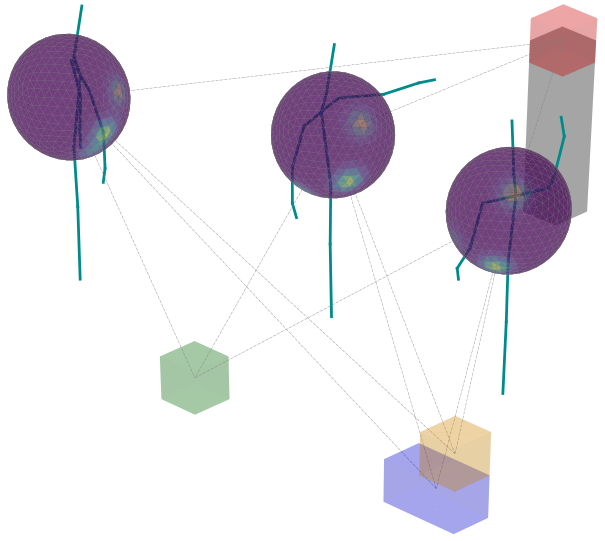
\includegraphics[scale=1.6,keepaspectratio]{fig/multi_robots.png}};
			\node at (0.0,4.1) [color=black] {\small \textbf{Interacttion and attention sharing}};
			\end{tikzpicture}
			\caption{The scene shows a situation where two agents are interacting about the orange object while a third agent is leaving the scene. Three other objects are present. The effect of stimuli projection in agents’ peripersonal is represented at a pre-selection level of attention in ego-spherical localization.}
			\label{fig:multi_robots}
		\end{center}
	\end{figure}

	As a continuation of previous research in which we proposed a model for tracking JA in HRI as a topology-based representation organized in a \textit{scale of jointness} \cite{chame2023top}, in this work we investigate the more fundamental aspect of attention selection and how such mechanism could allow the emergence of JA in human-robot interaction from top-down and bottom-up modulation processes. For this, as shown in Fig. \ref{fig:multi_robots}, we suppose unconstrained situations where agents can become interested in objects in the environment and eventually share attention and knowledge about them (e.g. situations like asking someone for direction or commenting about salient stimuli like a noise or an object). 
	
	Tacking into account the considerations above, we explore the concept of \textit{ego-sphere} \cite{albus1991} and propose the model named AEGO for tracking the attention focus of agents as represented from egocentric perspective, and resulting from on-board sensory acquisitions. For this, inspired by \textit{dynamic neural fields} (DNF) theory \cite{amari1977}, we model attention selection as a dynamical system process represented by neural fields networks with lateral connectivity. By addressing limitations on previous research, we show how neural excitatory and inhibitory interaction allows us to study the emergence of attention selection. Moreover, we show how the model can be used to track agents' interaction with peripersonal space, which is an interesting resource for HRI applications. 
	
	%Tacking into account the considerations above, we propose the model named JA-EGO for tracking the attention focus of agents as represented from egocentric perspective, and resulting from acquisitions of robot's on-board sensory. For this, we model the evolution of attention selection as a dynamical system process represented by a recurrent neural network inspired on \textit{dynamic neural fields} (DNF) theory \cite{amari1977}. Thus, JA-EGO can be used for track egocentric focus of attention from spherical localization references. 
	  	  
	This document is organized as follows: Section \ref{sec:previous} discusses previous works and argues how our contribution would help to advance the state of the art in the field. Section \ref{sec:model} presents the mathematical definition of the model and discusses theoretical assumptions behind it. Section \ref{sec:methodology} presents the methodology which consisted in: a) studying in simulation attention selection from top-down and bottom-up modulation processes, and showing potential applications, and b) conducting an experiment with the robot Pepper for a JA task based on proprioception, vision, basic natural language and Hebbian plasticity. Section \ref{sec:results} reports on the study’s results, and Section \ref{sec:conclusions} presents conclusions and future perspectives.
	  
%	For this, an egocentric perspective for localization is adopted where the robot is able to represent the dynamics of its own focus of attention in an sensory ego-spherical representation as well as tracking others' focus of attention. 
	
	
	\section{PREVIOUS WORK}
	\label{sec:previous}
	
	%Biological studies have pointed out to the existence of biological mechanisms to support essential cognitive functions such as attention, short-term memory, spatio-temporal sensory-motor coordination, and locomotion, among others.

	According to \cite{albus1991} an \textit{ego-sphere} consists of a two dimensional spherical map of the world as perceived by an observer placed at its center. This interesting idea has inspired several works in the field of robotics. A study by \cite{ruesch2008} has shown how attention and short-term memory can be modulated through saliency maps and allow the robot to explore the environment based on novelty. A work by \cite{bodiroza2011} focused on intuitive HRI, including the possibility of top-down modulation of attention. The aspect of information representation has also been studied in \cite{peters2009sensory}, so the ego-sphere has been implemented as a storage data-base indexed by spherical tessellation mapping. Other contributions could be mentioned (e.g. \cite{grotz2017}, \cite{marques2022}).%Other contributions based on these ideas could be mentioned (e.g. \cite{grotz2017}, \cite{marques2022}).
	
	
	To our knowledge, previous research has not explored sufficiently the aspect of interaction dynamics between locations represented in the ego-sphere, and considered at most basic forms of interaction spread between nodes. Moreover, excluding saliency map approaches (e.g. \cite{ruesch2008}), the dynamics of attention was modeled as a process governed by knowledge represented in the form of production rules, where the possibility of compositionality from low-level sensory to higher-level decision space has been of less importance. 
	 
	
	%in the field have achieved impressive results by exploring attention saliency in sensory egocentric representations under the effect of modulation processes (e.g. bottom-up \cite{ruesch2008} and top-down \cite{bodiroza2011}). Although most research have considered environment exploration tasks, so the robot can focus on learning new things based on novelty, some have studied social cognition or joint attention tasks inspired on psychological theories of attention (e.g. \cite{ruesch2008}). 
	
	
	
	%Moreover, when resorting to alternative forms of knowledge representation, generality is lost and the possibility of well stablished    
	
	 %as from representation in the same space where attention selection is done. We believe that this is an important limitation, when considering the possibility of investigating compositionality in joint attention as a descending (top-down) generative process combined with an ascending (bottom-up) saliency process, susceptible of study as a dynamical system.   
	
	Another limitation of previous research is considering the robot as the only one in interaction given with embodied sensory ego-spherical representations, so data coming from human agents is mostly represented in the robot's perspective. In our opinion, this would be a too egocentric approach for HRI. We believe that when keeping track of embodied relations between agents and objects in the environment as a distributed dynamical system, the robot could take decisions and behave without relying too much on environment modeling, from the emergence of attention from instantaneous interaction. Hence, we propose that attention selection is tracked simultaneously from participants' egocentric perspective. 
	 
	Previous works in our research teams also constituted relevant steps in the direction of developing the current study, which is worth mentioning. In \cite{heikkila2019} JA in HRI was studied for providing guidance in a shopping mall. Other works explored the concept of \textit{joint action} \cite{belhassein2022} and \textit{situation assessment} from perspective taking \cite{sallami2019}. In \cite{chame2016} an ego-cylindrical selection mechanism for attention was proposed for autonomous positioning with respect to objects in the environment. In \cite{chame2023top} the model TOP-JAM was proposed for tracking JA in HRI from allocentric references.  %\textcolor{orange}{[Many papers from the RIS team could be cited: human-aware planning, JA ... To be confirmed with Rachid]}.
	
	%Our previous research has also constituted relevant steps in the direction of developing the current study which is worth mentioning. In \cite{chame2016} an ego-cylindrical selection mechanism for attention was proposed for autonomous positioning with respect to objects in the environment. In \cite{chame2023top} the model TOP-JAM was proposed as a means for JA tracking in HRI from allocentric references. In \cite{heikkila2019} JA in HRI was studied for providing guidance in a shopping mall. Other related works studied \textit{joint action} and situation assessment from perspective taking \cite{sallami2019}. %\textcolor{orange}{[Many papers from the RIS team could be cited: human-aware planning, JA ... To be confirmed with Rachid]}.
	 
	To summarize, differently from previous approaches we propose to model attention for HRI in neural dynamic fields networks for tracking the influence of three important sources on attention selection: a) bottom-up stimulation, b) top-down modulation, and c) local interactions from inhibitory and excitatory synapse. We present in the next section the mathematical foundations of this model which we named AEGO. In Section \ref{sec:methodology} we show how AEGO is suited for investigating joint attention in HRI.
	
	% 
	
	
	%More importantly, attention clues from the human are not processed in the same representation space
	
	%attention processes dynamics has not been 
	
	%the body posture of the human has not being considered as an source of information for the robot attention process. Moreover, the sensory ego-sphere has been proposed as a computational data structure which does not represents directly the focus of attention of participants, neglecting thus the dynamics of interaction, consisting mostly in a data storage repository indexed by tessellation spherical mapping (see \cite{peters2009sensory}). 
	
	
	
	
	%\cite{ruesch2008}
	
	%The problem of placement of the egocentric localization reference is not trivial and would greatly depend on the task at hand.   
	
	%The origin of the ego-cylinder can be fixed to different parts of the body. There is no agreement in the literature on the placement for this structure.
	
	
	 %... in the field of cognitive robotics, the work by \cite{peters2009sensory} has proposed a data structure in the form of a sensory ego-sphere located at the robot base frame as a mediating interface between sensors and cognitive processes. 
	 
	%The work by \cite{chame2016} has proposed a sensory ego-cylindrical information fusion mechanism for egocentric localization allowing the robot to autonomous position with respect to object in the environment based on embodied representations. 
	
%	\begin{figure}[h!]
%		\begin{center}
%		\begin{tikzpicture}
%		\node [] at (0,0){
%			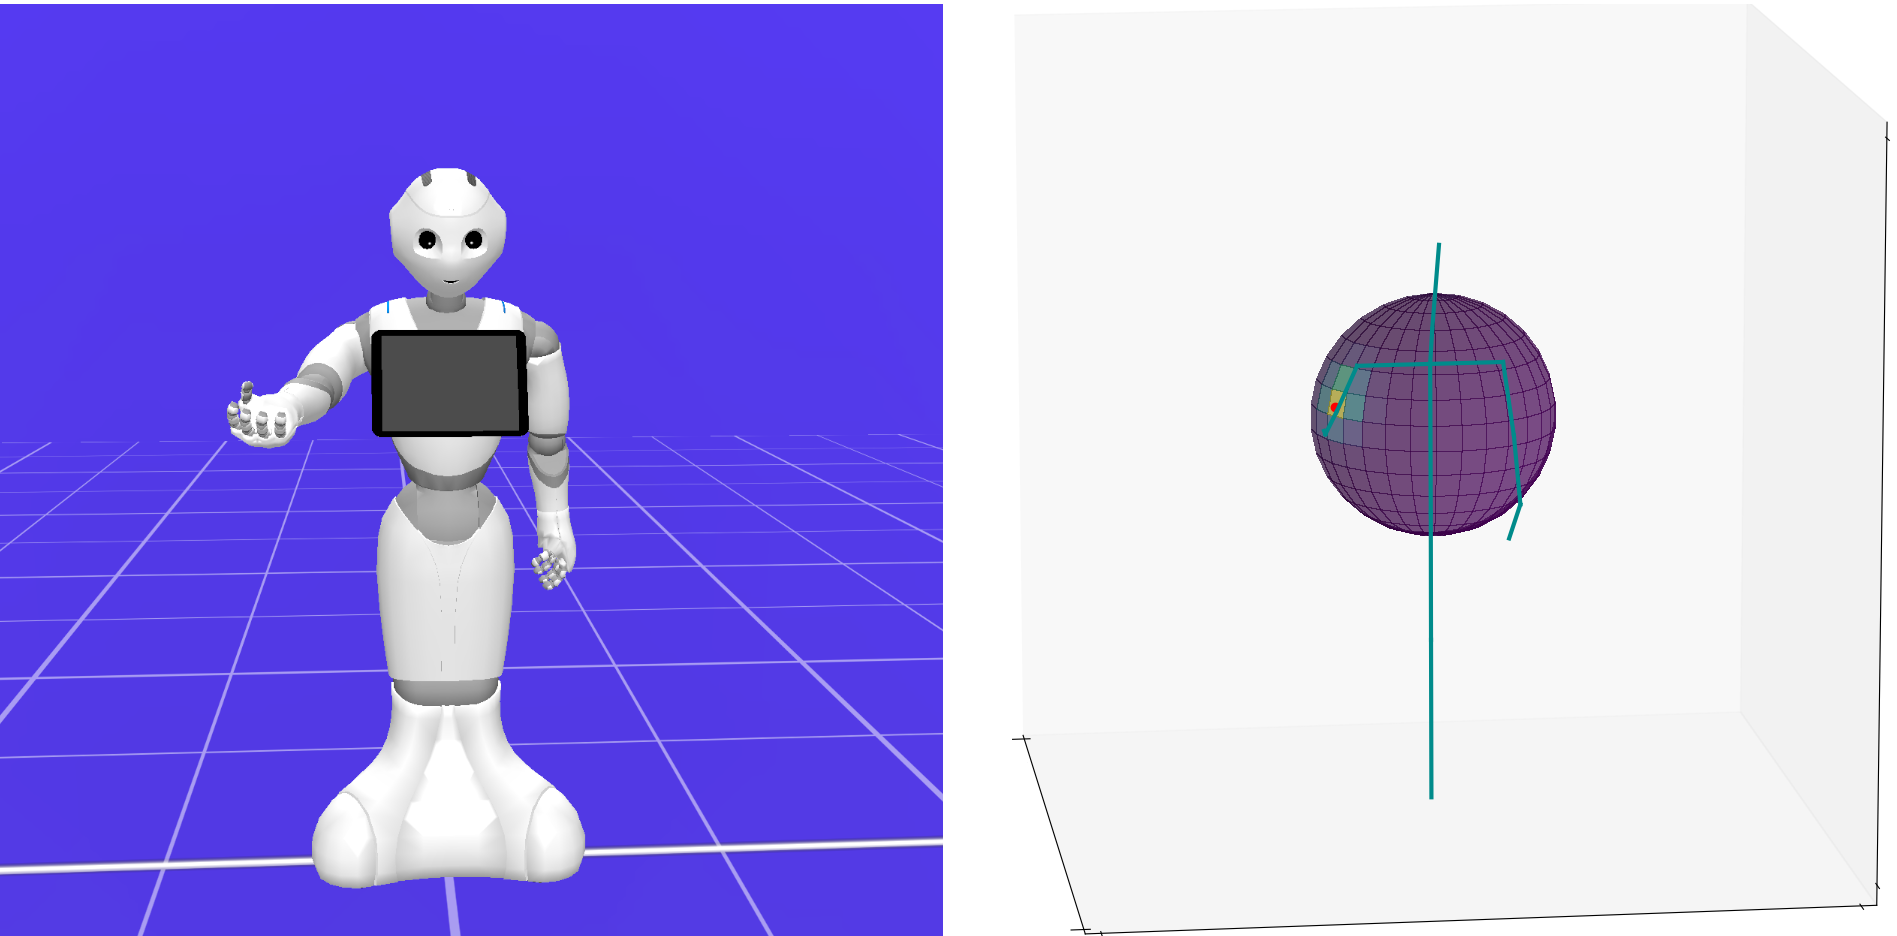
\includegraphics[scale=0.5,keepaspectratio]{fig/robot_pointing.png}};
%		\node at (0.0,2.4) [color=black] {\small \textbf{The robot sensory ego-sphere}};
%		\end{tikzpicture}
%		\caption{Left: the robot is pointing to a location in the space. Right: the attention state of the robot is shown as the activation of the neural network representing the sensory ego-sphere, as stimulated by the intersection of the forearm direction with by the sensory ego-sphere.}
%		\label{fig:robot_pointing}
%		\end{center}
%	\end{figure}

	
	\section{THE MATHEMATICAL MODEL}	
	\label{sec:model}
	
	Theoretical models of visual attention, such as \textit{feature integration theory} (FIT) \cite{treisman1980}, have described attention as a multi-level information fusion process. According to FIT, at a pre-attention level the perceptual system receives from separate maps feature salience information (e.g., color, edges, shapes), which are lately combined at an attention selection stage. A bio-inspired architecture has been proposed from FIT in \cite{koch1985} and implemented in \cite{itti1998}, with applications in robotics (e.g. autonomous navigation based on vision \cite{siagian2014}).

	\begin{figure}[h!]
		\begin{tikzpicture}
		\node [] at (0,0){
			\includegraphics[scale=0.37,keepaspectratio]{fig/model.eps}};
		\node at (0.0,3.0) [color=black] {\small \textbf{AEGO architectural view}};
		\end{tikzpicture}
		%\fcolorbox{white}{white}{
		%\includegraphics[scale=0.38]{model.eps}
		%}
		\caption{The model AEGO takes as inputs rough estimations on the objects' locations with respect to egocentric frames of reference, proprioceptive and basic natural language inputs. This information excites the attention pre-selection layer $\mathbf{u}$ (see Eq. \eqref{eq:pre-sel}), which provides input to the selection layer $\mathbf{a}$ (see Eq. \eqref{eq:sel}). In layer $\mathbf{k}$ (see Eq. \eqref{eq:out}) the model outputs the probability of focusing on a particular stimulus. Under top-down modulation, focused attention can influence pre-selection as a feedback process.}
		\label{fig:AEGO}
	\end{figure}

	%Let the agent's peripersonal space be represented by a localization topology defined by a vertex set, resulting from the tessellation of an icosahedron polyhedron, which approximates a spherical region around the agent. 
	This work proposes a model of attention selection inspired by FIT and DNF theory. However, we study not only visual information but consider other sources of stimulation. Thus, attention is modeled in an ego-spherical representation encoded by dynamic neural fields at a pre-attention phase, receiving stimulation from top-down and bottom-up processes, and synaptic interaction. In a subsequent phase, attention selection results from competition in synaptic interaction. The architectural view of the model is illustrated in Fig. \ref{fig:AEGO}. The mathematical definition of the model \footnote{\scriptsize \textbf{Notation.} Matrices and vectors are represented in bold, indexes are represented as subscripts (e.g. the $i^{\mathrm{th}}$ element of a vector $\mathbf{a}$ is denoted $\mathbf{a}_{i}$). Network layers are vectors. Matrices are represented in capital letter, the colon character represents the $i^{\mathrm{th}}$ row or column of a matrix (e.g. $\mathbf{A}_{i:}$ for columns and $\mathbf{A}_{:i}$ for rows). Position and orientation vectors are in 3D Cartesian space. The projection of a point $\mathbf{p}$ in the ego-sphere surface is denoted $\mathbf{\hat{p}}$.} is detailed next.
	
	
	\subsection{Pre-attention phase}
	Let the activation of the $i^\mathrm{th}$ neuron encode the dynamics of stimulation affecting a location  $\mathbf{x}_i$ in 3D Cartesian coordinates at a polyhedron surface representing the agent's ego-space, such that 
		
	\begin{equation}
	\tau_\mathrm{u} \dot{\mathbf{u}}_{i(t)} = -\mathbf{u}_{i(t-1)} + q_\mathrm{u} + \sum_{j}^{} (\mathbf{U}_{ij}+\epsilon)\mathbf{u}_{i(t-1)} + \mathbf{s}_{i(t,\Xi)} 
	\label{eq:pre-sel}
	\end{equation}

	According to the principle of local interconnections \cite{samsonovich97}, the interaction strength $\mathbf{U}_{ij}$ between neurons $i$ and $j$ is selected so proximal locations have stronger interaction. Hence, multivariate Gaussian weights are selected, such that
	
	\begin{equation}
		\mathbf{U}_{ij}(|\mathbf{x}_i-\mathbf{x}_j|) = \frac{\mathrm{exp}\left(-\frac{1}{2} (\mathbf{x}_i-\mathbf{x}_j)^{\mathrm{t}}\mathbf{\Sigma}^{-1}(\mathbf{x}_i-\mathbf{x}_j)\right)}{\sqrt{2\pi^{3}|\mathbf{\Sigma}|}}	
	\label{eq:pre-sel-syn}
	\end{equation}
	
	The term $\mathbf{s}_{i(t,\Xi)}$ represents the stimulation received at time instant $t$ affecting the ego-space locations $\Xi$. As it is going to be detailed in Section \ref{sec:methodology}, this term models stimulation from both top-down and bottom-up processes. Finally, in Eq. \eqref{eq:pre-sel} $q_\mathrm{u}$ corresponds to the activation resting state, $\tau_\mathrm{u}$ is the a time constant, and $\epsilon$ is a global inhibition factor affecting lateral interactions between neurons.
	 
	\subsection{Attention selection phase}
	
	Let the activation of the $i^\mathrm{th}$ neuron represent the dynamics of an attention selection process at a particular location in the ego-space, such that 
	
	\begin{equation}
	\tau_\mathrm{a} \dot{\mathbf{a}}_{i(t)} = -\mathbf{a}_{i(t-1)} + q_\mathrm{a} + \sum_{j}^{} \mathbf{A}_{ij}f\left(\mathbf{a}_{(t-1)}, \mathbf{u}_{(t)}\right) 
	\label{eq:sel}
	\end{equation}
	
	\noindent Inhibitory neural interaction has been associated with selection mechanisms \cite{schoner2016}. Thus, we propose to model lateral interaction $\mathbf{A}_{ij}$ between neuron $i$ and $j$ such that

	\begin{equation}
	\mathbf{A}_{ij}(|\mathbf{x}_i-\mathbf{x}_j|) = 1 - \varphi\mathbf{U}_{ij}	
	\label{eq:sel-syn}
	\end{equation}
	
	\noindent with $\varphi = \mathrm{max}(\mathbf{U}_{i:})^{-1}$ a scaling factor. The activation function $f$ in Eq. \eqref{eq:sel} is defined so

	\begin{equation}
	f\left(\mathbf{a}_{(t-1)}, \mathbf{u}_{(t)}\right) = \mathrm{sigmoid} \left(\gamma_\mathrm{a} \left(\mathbf{a}_{i(t-1)} + \gamma_\mathrm{u} \mathbf{u}_{i(t)}\right)\right)
	\label{eq:sel-fa}
	\end{equation}
	
	\noindent being $\gamma_\mathrm{a}$ and $\gamma_\mathrm{u}$ gain constants.
	
	\subsection{Object focus output layer}
	
	Let the probability $\mathbf{k}_\mathrm{i(t)}$ of attending to the $i^\mathrm{th}$ object be modeled as the output layer, such that
	
	\begin{equation}
	\mathbf{k}_\mathrm{i(t)} = \mathrm{softmax}\left(\gamma_{\mathrm{k}}\sum_{j}^{} \mathbf{O}_{ij(t)}\mathbf{a}_{j(t)}\right)
	\label{eq:out}
	\end{equation}
	
	\noindent where $\mathbf{O}_{ij}(|\mathbf{\hat{p}}_i-\mathbf{x}_j|)$ is obtained from Eq. \eqref{eq:pre-sel-syn} with $\mathbf{\hat{p}}_i$ the projection of the object's center of mass in the ego-sphere, and $\gamma_{\mathrm{k}}$ a gain factor constant.
	
	%\tau\dot{u}_i(x,t) = -u_i(x,t) + h + s_i(x,t) + \sum\limits_{i=0}^{j=N-1} w(|x_i-x_j|)f\left(u\left(x_j,t\right)\right)


%	\noindent with the stimulation input $\mathbf{s}_{i(t)}$ defined such that
%	\begin{equation}
%	\mathbf{s}_{i(t)} = \sum_{o}^{} (\mathbf{W}_{ij}+\epsilon)\mathbf{u}_{i(t-1)} + \varsigma \mathbf{s}_{i(t)} 
%	\label{eq:pre-sel-input}
%	\end{equation}
	

%	Let a ego-sphere representation of sensory information be modeled by the following neural network architecture \cite{amari1977}.
%	
%		\begin{figure}[h!]
%		\begin{center}
%			\begin{tikzpicture}
%			\node [] at (0,0){
%				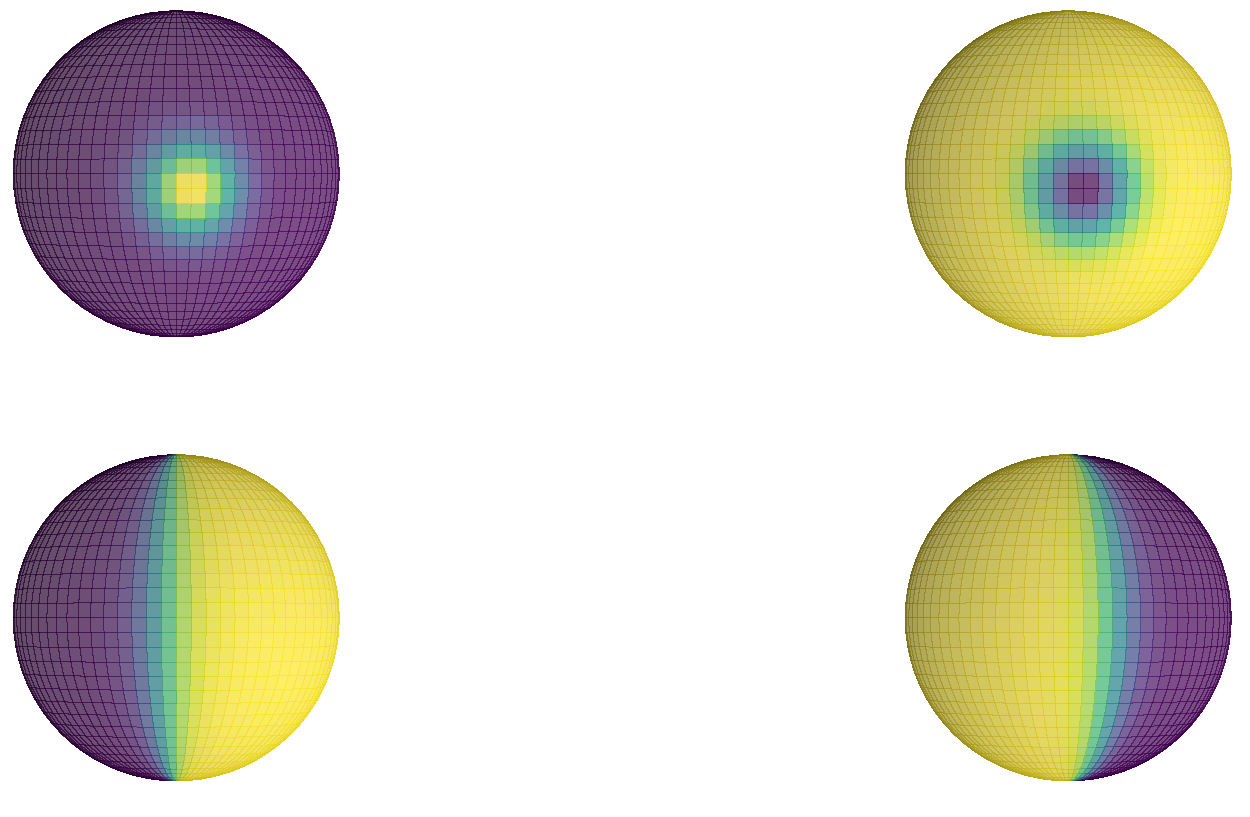
\includegraphics[scale=0.7,keepaspectratio]{fig/filters.png}};
%			\node at (0.0,2.6) [color=black] {\small \textbf{Pre-selection filters}};
%			\node at (-2.6,0.1) [color=black] {\scriptsize Point excitation};
%			\node at (2.6,0.1) [color=black] {\scriptsize Point inhibition};
%			\node at (-2.7,-2.4) [color=black] {\scriptsize Right-side excitation};
%			\node at (2.7,-2.4) [color=black] {\scriptsize left-side excitation};
%			
%			\end{tikzpicture}
%			\caption{Filters functions affecting the pre-selection phase.}
%			\label{fig:filters}
%		\end{center}
%	\end{figure}
%	
	
	\section{METHODOLOGY}
	\label{sec:methodology}

	Studies in simulations were designed for testing AEGO and analyzing potential application scenarios. We also conducted experiments with the robot Pepper for a JA task based on proprioception, vision, basic natural language and Hebbian plasticity. The details of the methodology are next.

	\subsection{Materials and Resources}
	
	The hardware components included a computer with 64 GB RAM memory, 11${}^\mathrm{th}$ Generation Intel\textsuperscript{\textregistered} Core\textsuperscript{\texttrademark} i9-11950H @ 2.60GHz × 16, and graphic card NVIDIA RTX A4000. The project counted on a humanoid robot Pepper, manufactured by Softbank Robotics. The software components were implemented in Python programming language versions 2.7 and 3, running in Ubuntu (20.04 LTS). The library MediaPipe version 0.10.3 was used to track the human posture from monocular vision. The library \textit{naoqi} version 2.5.7.1 was employed for the control programs and the software Choregraphe version 2.8.6.23 was used for simulations. 
	
	\subsection{Simulations}
	
	Table \ref{tab:params} presents common parameters for the model's layers described in Eqs. \eqref{eq:pre-sel}, \eqref{eq:sel} and \eqref{eq:out}. The state of the network is obtained through numerical integration by the Euler method with time-step $dt$. As shown in Fig \ref{fig:sim_objs}, six objects were simulated as bottom-up sources of stimulation to the agent. Topological search relying on the recognition of basic words was considered to explore top-down modulation of attention. %These situations are described below.
	
	%\setlength{\tabcolsep}{1.5pt}
	\renewcommand{\arraystretch}{1.2} % add a bit of more vertical space in table rows
	
	\begin{table}[h!]
		\caption{Common parameters for simulations}
		\label{tab:params}
		\begin{center}
			\begin{tabular}{p{3.2cm} p{4.2cm}}
				\cellcolor{darkcyan!20}\textbf{Parameter} & \cellcolor{darkcyan!20}\textbf{Value} \\
				Ego-sphere & 642 vertex, 1280 faces, radius 1 m\\
				%\cellcolor{gray!8}Ego-space faces number & \cellcolor{gray!8}1280 \\
				\cellcolor{gray!8}$\epsilon$ & \cellcolor{gray!8}0.0001\\
				$\tau_{\mathrm{u}}, \tau_{\mathrm{a}}$ & 200 ms\\
				\cellcolor{gray!8}$\mathbf{\Sigma}$ & \cellcolor{gray!8}$0.01\mathbf{I}_3$ \\
				$q_\mathrm{u}$ & -0.01 \\
				\cellcolor{gray!8}$q\mathrm{a}$ & \cellcolor{gray!8}-0.0001 \\
				$\gamma_{\mathrm{a}}$ & 50\\
				\cellcolor{gray!8}$\gamma_\mathrm{u}$ & \cellcolor{gray!8}2.5\\
				%$\gamma_\mathrm{n}$ & 15.5 \\
				$\gamma_\mathrm{k}$ & 250\\
				\cellcolor{gray!8}$dt$ & \cellcolor{gray!8}50 ms\\
			\end{tabular}
		\end{center}
	\end{table}
	
		\begin{figure}[h!]
			\begin{center}
			\begin{tikzpicture}
			\begin{scope}[scale=0.7]
			\node [] at (0,0){
				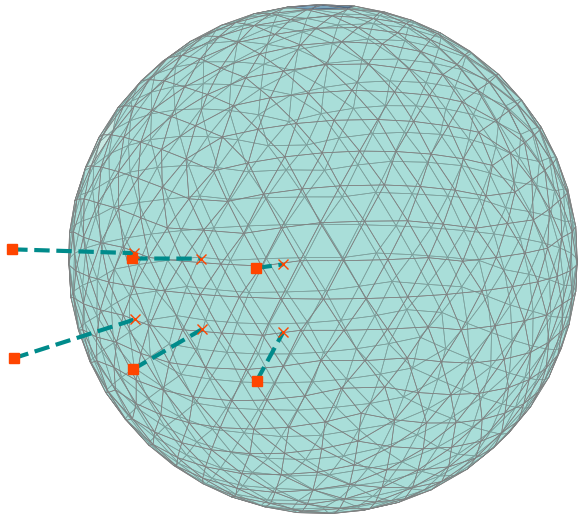
\includegraphics[scale=0.8,keepaspectratio]{fig/sim_objs.png}};
			\begin{scope}[shift={(3.2, -1.8)}]
			\draw[line width=1pt,darkcyan,-stealth](0.1,0)--(-0.5,-0.5) node[anchor=north east]{x};
			\draw[line width=1pt,darkcyan,-stealth](0.1,0.0)--(-0.9,0) node[anchor=north east]{y};
			\draw[line width=1pt,darkcyan,-stealth](0.1,0)--(0.1,1) node[anchor=north east]{z};
			\end{scope}			
			\node at (0.0,3.2) [color=black] {\small \textbf{Simulated bottom-up stimulation}};
			\begin{scope}[shift={(-0.8, 0.1)}, scale=1.7]
			\node at (0.2,-0.9) [color=red!70] {\small $\mathbf{p}_1$ };
			\node at (0.2,-0.25) [color=red!70] {\small $\mathbf{p}_2$ };
			\node at (-0.5,-0.85) [color=red!70] {\small $\mathbf{p}_3$ };
			\node at (-0.5,-0.2) [color=red!70] {\small $\mathbf{p}_4$ };
			\node at (-1.1,-0.75) [color=red!70] {\small $\mathbf{p}_5$ };
			\node at (-1.1,-0.15) [color=red!70] {\small $\mathbf{p}_6$ };
			\end{scope}
			\begin{scope}[shift={(0.3, 0.5)}, scale=1.7]
			\node at (-0.05,-0.7) [color=black!70] {\small $\mathbf{\hat{p}}_1$ };
			\node at (-0.15,-0.17) [color=black!70] {\small $\mathbf{\hat{p}}_2$ };
			\node at (-0.50,-0.67) [color=black!70] {\small $\mathbf{\hat{p}}_3$ };
			\node at (-0.55,-0.15) [color=black!70] {\small $\mathbf{\hat{p}}_4$ };
			\node at (-0.85,-0.63) [color=black!70] {\small $\mathbf{\hat{p}}_5$ };
			\node at (-0.9,-0.13) [color=black!70] {\small $\mathbf{\hat{p}}_6$ };
			\end{scope}
			\end{scope}	
			\end{tikzpicture}
			\caption{Bottom-up stimulation at six locations in the sensory ego-space. The objects' estimated center of mass coordinates $\mathbf{p}_i$ and projection $\mathbf{\hat{p}}_i$ on the ego-sphere are shown. To improve visualization, the frame of reference located at the ego-sphere's center is shown at bottom-right.}
			\label{fig:sim_objs}
			\end{center}
		\end{figure}
				
	\subsubsection{Focusing on named objects}
	
	we investigated the possibility of attending to a specific object as modulated by top-down processes. For this, it is assumed that the agent is able to track and recognize objects in the scene while associating unique words for addressing them. A numerical ID could serve this purpose. Thus, once the human says for instance "three", attention should be directed to stimuli which project around location $\mathbf{\hat{p}}_3$ (see Fig. \ref{fig:sim_objs}). For this, the term $\mathbf{s}_{i(t,\Xi)}$ in Eq. \eqref{eq:pre-sel} can be set so
	
	\begin{equation}
	\mathbf{s}_{i(t,\Xi)} = \sum_{j}^{} \gamma_{\mathrm{o}j}\mathbf{O}_{ij(t)}\left(|\mathbf{\hat{p}}_{j(t)} - \mathbf{x}_{i(t)}|\right)
	\label{eq:sim1}
	\end{equation}
	
	Interest to objects is modeled through the gain $\gamma_{\mathrm{o}j}$. For bottom-up saliency  $\gamma_\mathrm{bu} = 0.9$ for all detected objects, whereas for top-down modulation it is set to $\gamma_\mathrm{td} = 30\gamma_\mathrm{bu}$. Once a particular object's name is heart at time $t_\mathrm{w}$, it stimulates the model through a unit step function $\lambda = f(t_\mathrm{w}, t_\mathrm{w}+\delta_\mathrm{t})$ with duration $\delta_\mathrm{t} = 1\ \mathrm{sec}$, such that
	
	 \begin{equation}
	 \gamma_{\mathrm{o}j} = \lambda\gamma_\mathrm{td}+ (1-\lambda)\gamma_\mathrm{bu}
	 \label{eq:sim1-step}
	 \end{equation}
	
	\noindent The local influence of stimuli on the neural field $\mathbf{O}_{ij(t)}$ is set conforming to Eq. \eqref{eq:pre-sel-syn}.
	
	\subsubsection{Searching around objects} this simulation considered interactions based on perspective-taking, where someone indicates a topological reference in another's perspective, such as turning attention to a stimulus at \textit{right}, \textit{left}, \textit{above} or \textit{below}; which are words recognized by the robot. Thus, let $\mathbf{s}_{i(t,\Xi)}$ in Eq. \eqref{eq:pre-sel} be modeled such that
	
	\begin{equation}
	\mathbf{s}_{i(t,\Xi)} = \sum_{j}^{} f\left(\gamma_\mathrm{r}m_{(t)}\right)\ g\left(\left|\boldsymbol{\hat{\mu}}_{(t)} - \mathbf{x}_{i(t)}\right|\right)
	\label{eq:sim2}
	\end{equation}
	\noindent where $f(.)$ is the sigmoid function with $\gamma_\mathrm{r}$ representing a gain constant and $g(.)$ is the multivariate Gaussian function (see Eq. \eqref{eq:pre-sel-syn}). The coordinates of the projection $\boldsymbol{\hat{\mu}}$ on the ego-sphere, which corresponds to instantaneous attention selection, are obtained so 
	
	\begin{equation}
	\boldsymbol{\hat{\mu}}_{(t)} = \sum_{i}^{}\mathbf{k}_\mathrm{i(t-1)}\mathbf{\hat{p}}_{i(t)}
	\label{eq:sim2-mu}
	\end{equation}
	
	It is interesting noticing that, by receiving feedback from the output layer $\mathbf{k}_\mathrm{i(t-1)}$ at the previous time step (see Eq. \eqref{eq:out}), a local search can be set if the agent is actually focusing on a particular object. For the case of horizontal search, the point's  projection $y$ coordinate is considered, whereas for vertical search the $z$ coordinate would be relevant (see Fig. \ref{fig:sim_objs}). Hence, $m_{(t)}$ in Eq. \eqref{eq:sim2} is set such that
	
	\begin{equation}
	m_{(t)} = 
	\left\{
	\begin{split}
	\boldsymbol{\hat{\mu}}_{\mathrm{y}(t)}- \mathbf{\hat{p}}_{j\mathrm{y}(t)} & : \mathrm{``right"}\\
	\mathbf{\hat{p}}_{j\mathrm{y}(t)} - \boldsymbol{\hat{\mu}}_{\mathrm{y}(t)}& : \mathrm{``left"}\\
	\boldsymbol{\hat{\mu}}_{\mathrm{z}(t)}- \mathbf{\hat{p}}_{j\mathrm{z}(t)} & : \mathrm{``above"}\\
	\mathbf{\hat{p}}_{j\mathrm{z}(t)} - \boldsymbol{\hat{\mu}}_{\mathrm{z}(t)} & : \mathrm{``below"}\\
	\end{split}\right.
	\label{eq:sim2-m}
	\end{equation}
	
	\noindent Similarly to previous scenario, the gain $\gamma_{\mathrm{o}j}$ is set conforming to Eq. \eqref{eq:sim1-step} with duration $\delta_\mathrm{t} = 1\ \mathrm{sec}$. 
	
	\subsubsection{Losing interest in something} the situation considered here is the agent's loss of interest to an object form receiving negative feedback from the human. For this, inhibitory feedback from the selection layer $\mathbf{a}_{(t-1)}$ is provided to the pre-selection layer $\mathbf{u}_{(t)}$ (see Eqs. \eqref{eq:pre-sel},\eqref{eq:sel}). The term $\mathbf{s}_{i(t,\Xi)}$ in Eq. \eqref{eq:pre-sel} is modeled with a gain constant $\gamma_\mathrm{n}= 0.75$ so
	
	\begin{equation}
	\mathbf{s}_{i(t,\Xi)} = -\mathrm{softmax}\left(\gamma_\mathrm{n}\mathbf{a}_{i(t-1)}\right)
	\label{eq:sim3}
	\end{equation}
	
	\noindent The gain $\gamma_{\mathrm{o}j}$ is set conforming to Eq. \eqref{eq:sim1-step} but the duration of stimulation is selected shorter for this case $\delta_\mathrm{t} = 0.5\ \mathrm{sec}$. 
		
	%next*(self._ut.softmax(15.5*self._u_sel))
	
	\subsection{Experiment}
	
	An interaction experiment was designed with the robot Pepper. Since the robot is capable of recognizing typical landmarks, some were attached to locations in the environment representing objects (see Fig. \ref{fig:exp_scene}). The robot is also capable of speech recognition within dialog context, so it was programmed to recognize the terms \textit{above}, \textit{below}, \textit{left}, \textit{right}, \textit{no}, \textit{one}, \textit{two}, \textit{three}, and \textit{four}. The ego-space was placed at the robot's \textit{Torso} frame, when in Stand-up posture. In this study we do not consider the possibility of rotation and translation of the ego-sphere (which would require geometrical remapping), so the experiment would correspond to situations of short interactions where participants talk about objects around. 
	
	%\textcolor{orange}{[I got until here ...]}
	The library MediaPipe was used to track the human skeleton and represent his/her ego-sphere, from the robot's on-board camera acquisitions. Thus, the robot was programmed to keep the human's full body in view during interaction. The human provided feedback to the robot verbally or by pointing to locations in the environment. In order to track non-verbal focus of attention, the intersection of both forearms with the ego-sphere (once reaching a certain height with respect to the torso) was considered as a measure of interest to the surrounding. As for the robot, the human's ego-sphere is assumed to be fixed during interaction. 
	
	To provide the robot with perspective-taking, the human was instructed to imitate it in a learning stage, so the robot points at each object during 5 seconds, names the object being pointed, and activates instantaneously a Hebbian plasticity rule to learn how the human's ego-sphere state relates to it own while sharing attention about that particular object. Hence, the synaptic weights are learned such that
	
	\begin{equation}
	\mathbf{H}_{oij(t)} = \mathbf{H}_{oij(t-1)} + \alpha \sum_{k}\sum_{j}\mathbf{k}_{\mathrm{r}o(t)}\mathbf{a}_{\mathrm{r}i(t)}\mathbf{a}_{\mathrm{h}j(t)}
	\label{eq:hebb_rule}
	\end{equation}	
	
	\noindent with $\alpha$ the learning rate. During the interaction stage, a source of stimulation coming from the human's behavior, so the term $\mathbf{s}_{i(t,\Xi)}$ in Eq. \eqref{eq:pre-sel} is modeled with gain $\gamma_{\mathrm{h}}$ so
	
	\begin{equation}
	\mathbf{s}_{i(t,\Xi)} = \gamma_{\mathrm{h}}\sum_{o}\sum_{j}\mathbf{H}_{oij(t)}\mathbf{a}_{\mathrm{h}j(t)}
	\label{eq:hebb_stim}
	\end{equation}	
	
%		
	\section{RESULTS}
	\label{sec:results}
	
	Globally, the studies in simulation showed the possibility of representing bottom-up saliency and top-up modulation of attention at the pre-selection layer. Let us take for instance simulations of the embodied operators to illustrate this point. As shown in Fig \ref{fig:sim2}, by considering feedback from the agent's focus of attention at the output layer, it was possible to modulate neural dynamics at related regions of the ego-sphere for helping the agent to respond to embodied references in verbal communication.  
	
	Figure \ref{fig:sim2-around} shows 60 seconds of the simulated interaction. Here, the operators \textit{left}, \textit{right}, \textit{above} and \textit{below} were employed so the agent could focus on the six stimuli one at a time. Similar results were obtained for the other two operations proposed \textit{focusing on named objects} and \textit{losing interest in something}. It is interesting noticing in the plot at the center how attention selection is obtained through a competition process, resulting from inhibitory neural interaction. 


	\begin{figure}[h!]
		\begin{center}
			
		\begin{tikzpicture}
		\node [] at (0,0){
		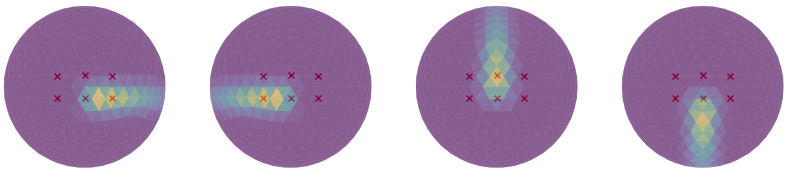
\includegraphics[scale=1.3,keepaspectratio]{fig/sim2_around_op.png}};
		\node at (0.0,1.4) [color=black] {\small \textbf{Embodied operators}};
		\node at (-3.4,-1.2) [color=black] {\scriptsize \textit{left}};
		\node at (-1.1,-1.2) [color=black] {\scriptsize \textit{right}};
		\node at (1.2,-1.2) [color=black] {\scriptsize \textit{above}};
		\node at (3.4,-1.2) [color=black] {\scriptsize \textit{below}};
		\end{tikzpicture}
		\end{center}
		\caption{Operators described in the simulation scenario \textit{searching around objects}. The top-down modulation of attention is shown after instantaneous recognition of the words \textit{left}, \textit{right}, \textit{above}, and \textit{below} see (Eq. \eqref{eq:sim2}), relative to the location $\mathbf{\hat{p}}_3$ in Fig. \ref{fig:sim_objs}).}
	\label{fig:sim2}
	\end{figure}

\begin{figure}[h!]
	\begin{center}
		\begin{tikzpicture}
		\node [] at (0,0){
			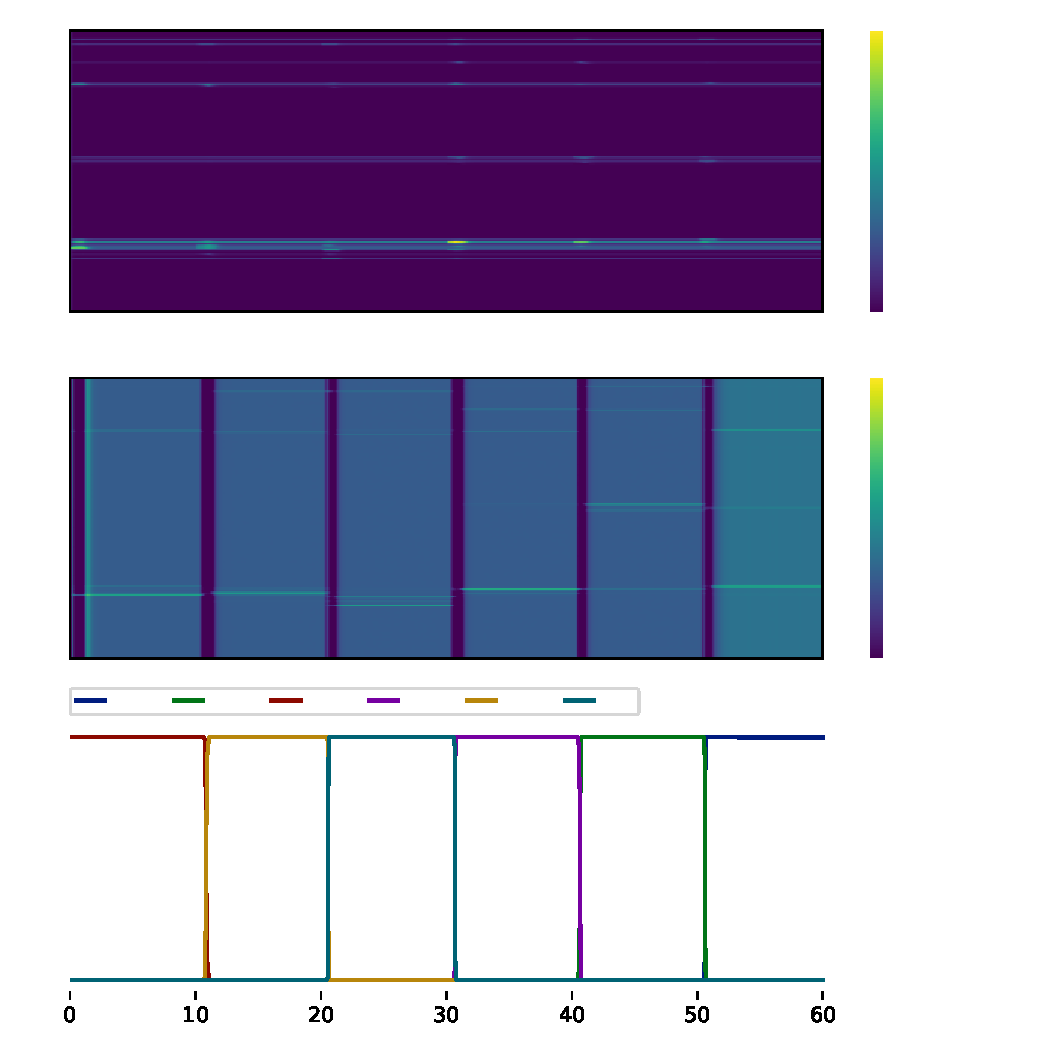
\includegraphics[scale=0.5,keepaspectratio]{fig/sim2_around.pdf}};
		\node at (0.0,4.6) [color=black] {\small \textbf{Searching around objects}};
		
		%maxval u_pre =  0.1
		%minxval u_pre =  -0.01						
		\draw (3.3,4.1) node[rotate=0,scale=1] { \tiny 0.1};
		\draw (3.3,1.85) node[rotate=0,scale=1] { \tiny -0.01};
		
		%maxval u_sel =  0.0011999622746858437
		%minxval u_sel =  -1.4
		\draw (3.3,4.1-2.9) node[rotate=0,scale=1] { \tiny 0.001};
		\draw (3.3,1.85-2.9) node[rotate=0,scale=1] { \tiny -1.4};
		
		\draw (-4.2,3) node[rotate=0,scale=1] { \scriptsize $\mathbf{u}_{(t)}$};
		\draw (-4.2,0) node[rotate=0,scale=1] { \scriptsize $\mathbf{a}_{(t)}$};
		\draw (-4.2,-3) node[rotate=0,scale=1] { \scriptsize $\mathbf{k}_{(t)}$};
		\draw (-0.5,-4.5) node[rotate=0,scale=1] { \scriptsize Time in seconds};
		\draw (-3.2,-1.5) node[rotate=0,scale=1] { \tiny $\mathrm{k}_{1}$};
		\draw (-2.5,-1.5) node[rotate=0,scale=1] { \tiny $\mathrm{k}_{2}$};
		\draw (-1.6,-1.5) node[rotate=0,scale=1] { \tiny $\mathrm{k}_{3}$};
		\draw (-0.8,-1.5) node[rotate=0,scale=1] { \tiny $\mathrm{k}_{4}$};
		\draw (0.0,-1.5) node[rotate=0,scale=1] { \tiny $\mathrm{k}_{5}$};
		\draw (0.8,-1.5) node[rotate=0,scale=1] { \tiny $\mathrm{k}_{6}$};
		
		\draw[color=black!80] (-3.85,-4) -- (-3.85,-1.8);
		\end{tikzpicture}
	\end{center}
	\caption{Focusing initially on object 3 (relative to $\mathbf{\hat{p}}_3$, see Fig. \ref{fig:sim_objs}), the agent switches attention to surrounding objects, from instantaneous recognition of words in the sequence: \textit{right} ($t=10$), \textit{above} ($t=20$), \textit{left} ($t=30$), \textit{left} ($t=40$) and \textit{below} ($t=50$). For more details, see Eqs. \eqref{eq:sim2}\eqref{eq:sim2-m}.}
	\label{fig:sim2-around}
\end{figure}

Concerning the interaction experiment with Pepper (see Fig. \ref{fig:exp_scene}), results showed that during the learning phase the human was able to learn the objects' name from the robot, whereas the robot was able to learn the body relation of the human to such objects. A total of six trials were recorded. It is important to mention that the human was only instructed to stand between the landmarks while facing the robot. No marks were attached to the floor to avoid rigorously determining the human’s position, thus introducing some variability in trials. Figure \ref{fig:exp_hebb} presents the comparison of attention modulation from learning in the first trial (see Eq. \eqref{eq:hebb_rule}), so object saliency is induced on other trials without re-enabling learning (see Eq; \eqref{eq:hebb_stim}). Thus, it can be noticed that the Hebbian plasticity rule was able to generalize for other trials in the experiment.

\begin{figure}[h!]
	\begin{center}
		
		\begin{tikzpicture}
		\node [] at (0,0){
			\includegraphics[scale=0.25,keepaspectratio]{fig/exp_scene.png}};
		\node at (0.0,3.6) [color=black] {\small \textbf{The experimental scene}};
		\end{tikzpicture}
	\end{center}
	\caption{Landmarks recognized by Pepper were fixed in the room for emulating objects. The human stood in front of the robot.}
	\label{fig:exp_scene}
\end{figure}

\begin{figure}[h!]
	\begin{center}
		
		\begin{tikzpicture}
		\node [] at (-0.7,0){
			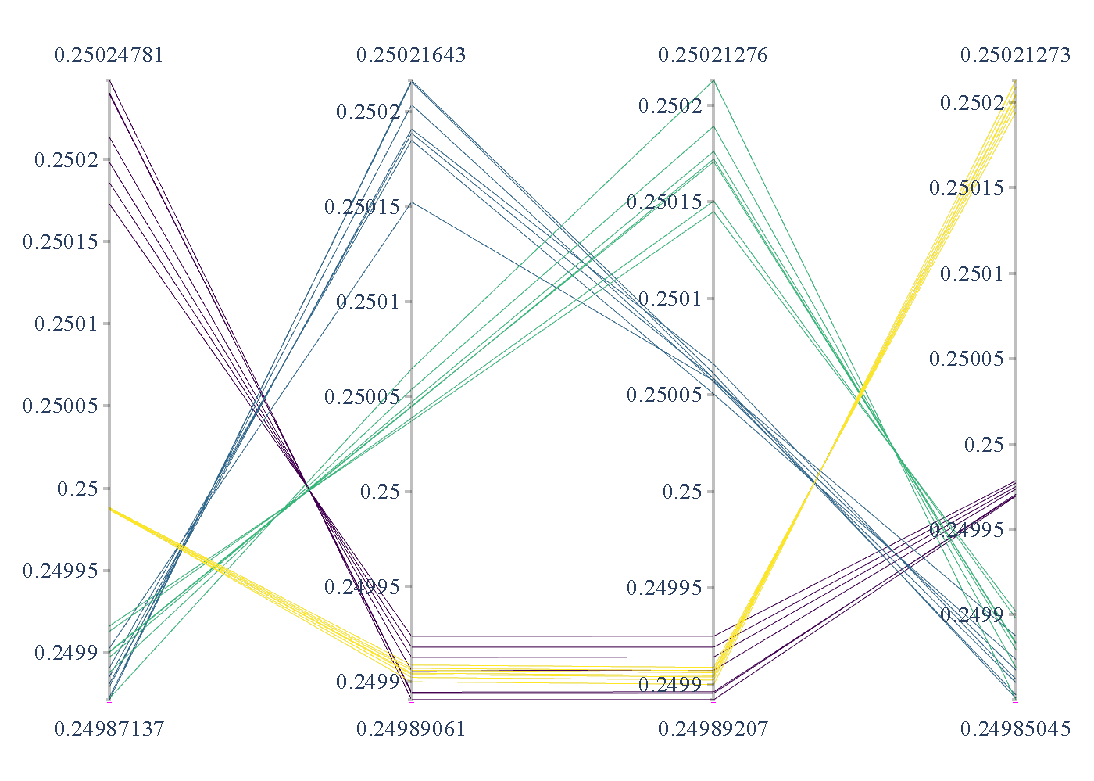
\includegraphics[scale=0.46,keepaspectratio]{fig/plot_generalisation.pdf}};
		
		\node at (-0.4,3.3) [color=black] {\small \textbf{Hebbian plasticity and generalisation}};
		
		% removing unwanted labels
		\filldraw[draw=white,color=white] (-5.0,2.5) rectangle (3.7,2.7);	
		\filldraw[draw=white,color=white] (-5.0,-2.5) rectangle (3.7,-2.7);	
		
		\node at (-4.2,2.7) [color=black] {\scriptsize Activity at $\mathbf{\hat{p}}_1$};
		\node at (-1.9,2.7) [color=black] {\scriptsize Activity at $\mathbf{\hat{p}}_2$};
		\node at (0.5,2.7) [color=black] {\scriptsize Activity at $\mathbf{\hat{p}}_3$};
		\node at (2.7,2.7) [color=black] {\scriptsize Activity at $\mathbf{\hat{p}}_4$};
		
		\node at (0.7-4.5,0.1-3.2) [color=black] {\scriptsize Human pointing at:};
		\filldraw[draw=black,color=hebb1] (0.0-2.5,0.0-3.2) rectangle (0.2-2.5,0.2-3.2);	
		\node at (0.7-2.5,0.1-3.2) [color=black] {\scriptsize Object 1};
		\filldraw[draw=black,color=hebb2] (0.0-1.0,0.0-3.2) rectangle (0.2-1.0,0.2-3.2);	
		\node at (0.7-1.0,0.1-3.2) [color=black] {\scriptsize Object 2};
		\filldraw[draw=black,color=hebb3] (0.0+0.5,0.0-3.2) rectangle (0.2+0.5,0.2-3.2);	
		\node at (0.7+0.5,0.1-3.2) [color=black] {\scriptsize Object 3};
		\filldraw[draw=black,color=hebb4] (0.0+2.0,0.0-3.2) rectangle (0.2+2.0,0.2-3.2);	
		\node at (0.7+2.0,0.1-3.2) [color=black] {\scriptsize Object 4};
		
		\node at (-4.9,0.2) [color=black] {\scriptsize $\mathbf{u}_{\mathrm{r}(t)}$};
		
		%\filldraw[draw=black,color=lightgray] (1,1) rectangle (1.2,1.2);		
		%\filldraw[draw=black,color=lightgray] (1,1) rectangle (1.2,1.2);
		%\filldraw[draw=black,color=lightgray] (1,1) rectangle (1.2,1.2);
		\end{tikzpicture}
	\end{center}
	\caption{The instantaneous state of the human focus of attention stimulates the robot's pre-selection layer, as described in Eq. \eqref{eq:hebb_stim}. Despite variability in positioning, after learning a single trial, the human's pointing gesture was able to modulate the robot's attention state for all remaining trials.}
	\label{fig:exp_hebb}
\end{figure}

Figure \ref{fig:exp_frames} shows a sequence of pointing gestures captured from the robots on-board camera. Both agent's ego-sphere were tracked on-line during the experience. In the situation depicted, the robot was observing the human after learning. Thus, the body posture of the human was able to modulate attention at a pre-selection level on the robot (see Eq. \eqref{eq:hebb_stim}), relative to stimuli salient in the environment. 

	\begin{figure}[h!]
	\begin{center}
		
		\begin{tikzpicture}
		\node [] at (0,0){
			%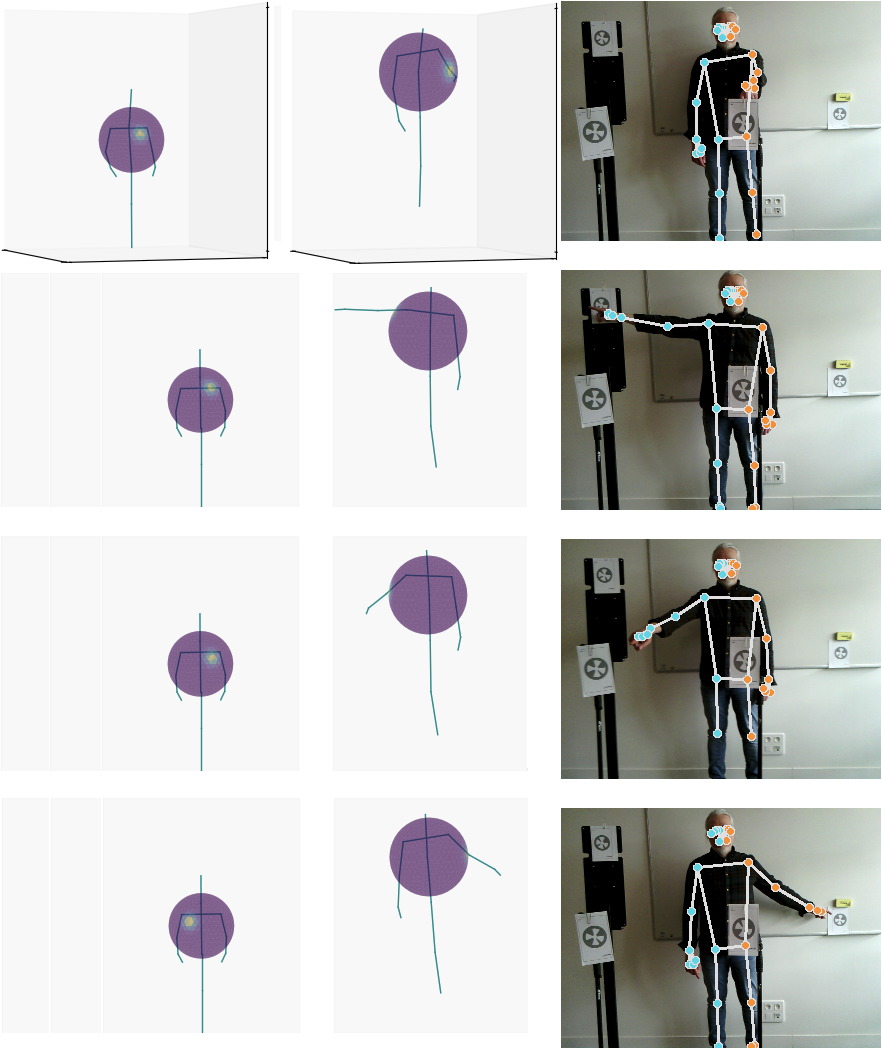
\includegraphics[scale=1.3,keepaspectratio]{fig/exp_frame_0.png}};
			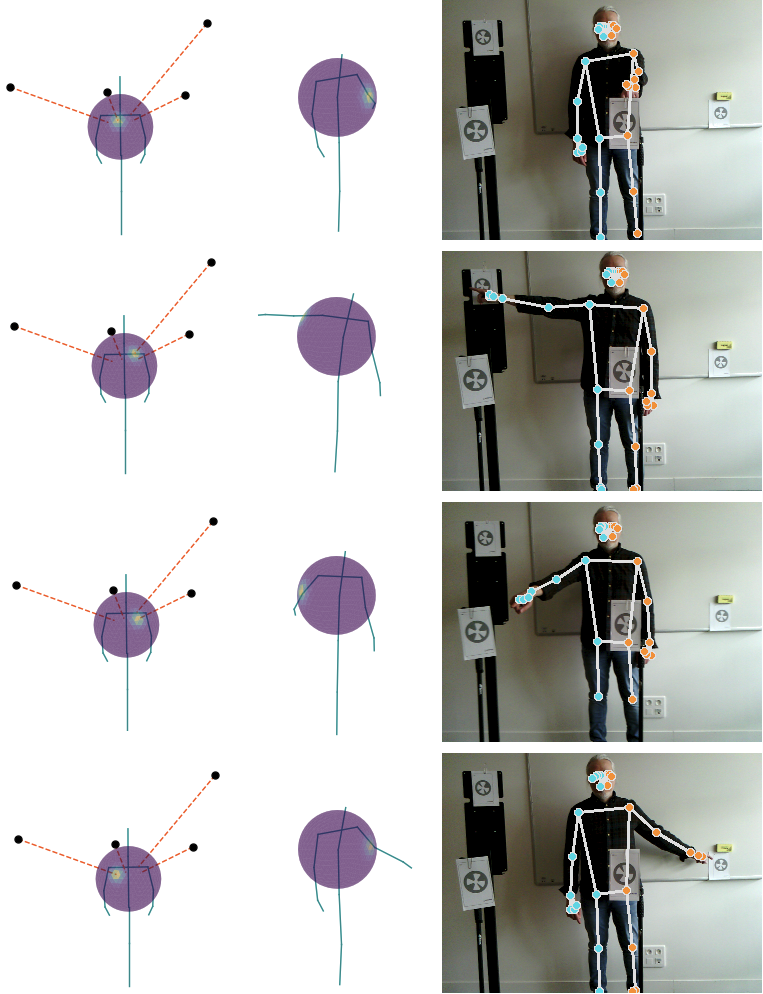
\includegraphics[scale=1.32,keepaspectratio]{fig/exp_frame_1.png}};
			%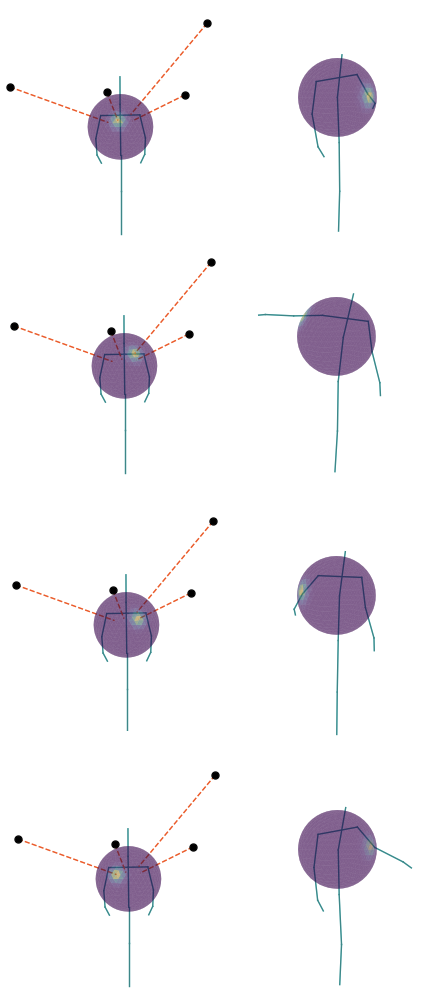
\includegraphics[scale=2.32,keepaspectratio]{fig/exp_frame_2.png}};
		\node at (-3.2,4.7) [color=black] {\scriptsize $\mathbf{p}_1$};
		\node at (-1.65,2.7) [color=black] {\scriptsize $\mathbf{p}_2$};
		\node at (-1.9,-1.0) [color=black] {\scriptsize $\mathbf{p}_3$};
		\node at (-4.0,-3.65) [color=black] {\scriptsize $\mathbf{p}_4$};
		\node at (0.0,6.0) [color=black] {\small \textbf{Interaction sequence}};
		\end{tikzpicture}
	\end{center}
	\caption{The ego-spheres are shown for the robot (left) and the human (center, rotated 160° around the $z$ axis to improve visualization). For the robot, projection rays of four landmarks are shown in red with estimated location in the scene in black. The human skeleton is tracked from the robot's camera (right) at about 10 Hz. Each row corresponds to pointing at a given landmark. After the learning phase, the human pointing behavior is able to stimulate locations in the robot's ego-sphere which also relate to landmark saliency. This helps  the robot to focus on such objects.}
	\label{fig:exp_frames}
\end{figure}
	
	\section{CONCLUSIONS}
	\label{sec:conclusions}
	
	This work originated from the interest of modeling attention selection and knowledge sharing in HRI from low level cognitive skills, so considering unstructured interaction situations encountered in everyday life. For this, the aspect of knowledge representation was carefully considered. From the literature revision, important limitations of previous works, which can be summarized as: a) not exploring in depth the aspect of interaction dynamics between locations represented in the ego-sphere, b) being a too egocentric approach for HRI by considering the robot as the only one in interaction given with embodied ego-spherical representations, and c) with very few exceptions, neglecting mostly the aspect of compositionality in knowledge representation.
	
	Consequently, we proposed a three-layered neural model to represent attention selection inspired by 4E cognition, FIT and DNF research. We named it AEGO and showed how bottom-up saliency, top-down generative modulation and lateral neural interaction allows tracking and representing the agents' focus of attention on-line as a distributed dynamical system. The model presents the advantage of being differentiable and is proposed in analytical form, so it could benefit from methods well established in the field of machine learning, as well as complement or enhance existing neural network models for tasks requiring attention tracking. 
	
	The results of simulations and experiments suggested that keeping track of embodied relations between agents and objects in the environment as a distributed dynamical system, and letting interaction structure those relations as an indivisible component of cognition, can be a promising approach for robots to be able to communicate and behave without facing the high cost of acquiring extensive knowledge about the environment. We showed how basic neural plasticity mechanisms in AEGO could be interesting for JA in HRI.
	
	Some topics, however, could not be investigated here and are left for future research. One aspect to be studied is the possibility on the robot's side to initiate JA by directing the head towards stimuli. Since tracking is done with the camera mounted on the head, the human would leave the field of view, hence some form of generative anticipation of human's attention would be required. Another important aspect to consider when sharing attention is social affordance. Thus, more complex forms of modulation in JA unfolding within a social context must be studied. 
	
	
	%Another issue that could not be studied is joint attention under rhythmic interaction. 
	
	%We believe that when keeping track of embodied relations between agents and objects in the environment and letting interaction structure those relations as an indivisible component of cognition, the robot can take decisions and show simple forms of adaptation and communication without relying too much on environment modeling, and that such processes rely importantly on attention sharing.
	
	% the emergence of attention from instantaneous interaction. Hence, we propose that attention selection is tracked simultaneously from participants' egocentric perspective. 
	
	
	
	
	\addtolength{\textheight}{-12cm}   % This command serves to balance the column lengths
	% on the last page of the document manually. It shortens
	% the textheight of the last page by a suitable amount.
	% This command does not take effect until the next page
	% so it should come on the page before the last. Make
	% sure that you do not shorten the textheight too much.
	
	%%%%%%%%%%%%%%%%%%%%%%%%%%%%%%%%%%%%%%%%%%%%%%%%%%%%%%%%%%%%%%%%%%%%%%%%%%%%%%%%
	
	
	
	%%%%%%%%%%%%%%%%%%%%%%%%%%%%%%%%%%%%%%%%%%%%%%%%%%%%%%%%%%%%%%%%%%%%%%%%%%%%%%%%
	
	
	
	%%%%%%%%%%%%%%%%%%%%%%%%%%%%%%%%%%%%%%%%%%%%%%%%%%%%%%%%%%%%%%%%%%%%%%%%%%%%%%%%
	%\section*{APPENDIX}
	
	%Appendixes should appear before the acknowledgment.
	
	\section*{ACKNOWLEDGMENT}
	
	This research was only possible with the collaboration of colleagues from the robotics teams of both LAAS-CNRS (project ANITI) and LORIA-CNRS (project Creativ’Lab).
	
	
	
	%%%%%%%%%%%%%%%%%%%%%%%%%%%%%%%%%%%%%%%%%%%%%%%%%%%%%%%%%%%%%%%%%%%%%%%%%%%%%%%%
	
	
	\bibliographystyle{acm}
	\bibliography{references}	
	
	
	
\end{document}
